\documentclass{article}

\usepackage{url}
\usepackage{graphicx}
\graphicspath{{figs/}}
\usepackage{subfigure}

\usepackage[utf8]{inputenc}
\usepackage[ngerman]{babel}

\usepackage{booktabs}
\usepackage{multirow}
\usepackage{pifont}
\usepackage{color}
\newcommand{\cmark}{\ding{51}}%
\newcommand{\xmark}{\ding{56}}%
\usepackage{listings}

\definecolor{blue}{rgb}{0,0,1}
\definecolor{violet}{rgb}{0.5,0,0.5} 
\definecolor{darkred}{rgb}{0.5,0,0}
\definecolor{darkblue}{rgb}{0,0,0.75}
\definecolor{darkgreen}{rgb}{0,0.5,0}

\lstset{%
  language=C,%
  morekeywords={constexpr,nullptr,size\_t,this,send,receive,\_\_global,\_\_kernel},%
  basicstyle=\ttfamily\small,%
  sensitive=true,%
  keywordstyle=\color{darkblue},%
  stringstyle=\color{darkgreen},%
  commentstyle=\color{violet},%
  showstringspaces=false,%
  tabsize=4,%
  numberstyle=\footnotesize,%
  xleftmargin=\parindent,%
  moredelim=[is][\color{red}]{|}{|},
  breaklines=true
}

\begin{document}

%don't want date printed
\date{}

\title{Verteilte Systeme Aufgabe 4 Konzept}

\author{
  Marian Triebe, Moritz Heindorf\\
  %Dept. Informatik, HAW Hamburg, Germany\\
  \{marian.triebe, moritz.heindorf\}@haw-hamburg.de
}

\maketitle

\section{Analyse der Aufgabenstellung}
Es soll ein Programm zur Zeitsynchronisation erstellt werden, dazu wird ein Zeitschlitzverfahren verwendet welche oft in echtzeitfähigen Systemen anzufinden sind. Zeitschlitze werden hierbei statisch bei Programmstart zugewiesen. Die Kommunikation zwischen den einzelnen Rechnern/Instanzen geschieht über UDP (Multicast).
Es existiert eine Master Instanz welche ein so genanntes \textit{Beacon} sendet, darauf hin beginnt eine neue \textit{Superframe}. In einem \textit{Superframe} senden alle Instanzen in Ihrem zugeteilten Zeitschlitz eine \textit{Slot-Nachricht}, das versenden soll genau in der Mitte des zugeteilten Zeitschlitzes geschehen. Die Anwendung soll später mit Lösungen von anderen Teams arbeiten können, deshalb sind die definierten Datenstrukturen aus der Aufgabenstellung zu verwenden.

\section{Aufbau der Programme}
Die Anwendung wird in C Programmiert werden und nur Support für Linux besitzen, da zum sicherstellen der korrekten Timings der \textit{HRTimer (High Resolution Timer)} des Linux Kernels eingesetzt werden soll. UDP ist zwingend notwendig um Nachrichten an alle Instanzen per Multicast ausliefern zu können. Der \textit{HRTimer} löst das Signal \textit{SIGALRM} aus, woraufhin eine neue Nachricht versendet wird. Beim Empfangen einer neuen Nachricht wird vom Socket \textit{SIGIO} ausgelöst. Es müssen Signalhandler für diese Signale implementiert werden.

\subsection{Superframe}
\begin{center}
\includegraphics[scale=.5]{Documents/frameformat.png}\\
\tiny Abbildung 1\\
\tiny Quelle: http://tiserver02.cpt.haw-hamburg.de/htm/vs.php?page=aufgabe4
\end{center}
Das Format der Superframe ist definiert und Abbildung 1 zu entnehmen. Die Superframe ist 100msec lang und setzt sich aus dem \textit{Beacon-Fenster} (20msec) gefolgt von einer Sicherheitspause von 4msec, 16*4msec Zeitschlitzen und einer 12msec Sicherheitspause zusammen.

\subsection{Beacon}
\begin{center}
\begin{lstlisting}
#define HOST_LEN 32
struct beacon {
  uint32_t frameNr;
  uint64_t timeShift;
  char host[HOSTLEN];
};
\end{lstlisting}
\tiny Listing 1\\
\end{center}
In Listing 1 ist die interne definition einer \textit{Beacon-Nachricht} dargestellt. Diese Nachricht soll dann als ASCII formatierte Nachricht in das Netzwerk gesendet werden. Der Aufbau dieses ASCII Strings ist der Aufgabenstellung entnommen und ist in Listing 2 definiert.
\begin{center}
\begin{lstlisting}
/*
	B<frameNr>:<timeShift>:<hostname>

    frameNr:    Fortlaufende Nummerierung des Frames.
    timeShift:  Tatsaechlicher Sendezeitpunkt des Beacons in nsec, relativ zum Startzeitpunkt des Frames.
    hostname:   ASCII-String, maximale Laenge: 32 Zeichen

    Beispiel:
        B218:2888685:Lab22
*/
\end{lstlisting}
\tiny Listing 2\\
\tiny Quelle: http://tiserver02.cpt.haw-hamburg.de/htm/vs.php?page=aufgabe4
\end{center}

\newpage
\subsection{Slot-Nachricht}
Die \textit{Slot-Nachricht} soll von der jeweiligen Instanz in der Mitte des zugeteilten Zeitschlitzes versendet werden. Die Nachricht soll als ASCII String versendet werden, die Zusammensetzung ist in Listing 3 definiert.

\begin{center}
\begin{lstlisting}
/*
D<slotnummer>:<hostname>

    slotnummer: Zahl 1 bis 16
    hostname:   ASCII-String, maximale Laenge: 32 Zeichen

    Beispiel:
        D9:Lab29
*/
\end{lstlisting}
\tiny Listing 3\\
\tiny Quelle: http://tiserver02.cpt.haw-hamburg.de/htm/vs.php?page=aufgabe4
\end{center}

\section{Mögliche Probleme}
\begin{itemize}
	\item Nicht korrekte Verwendung der Datenstrukturen einzelner Teams
	\item Senden zu falschen Zeiten (nicht im eigenen Slot)
	\item Delay durch Signallaufzeiten (Im Labor irrelevant)
	\item Ausbleiben des Beacons
\end{itemize}

\section{Grober Ablauf eines Beacons}
Das hier dargestellte Sequenzdiagramm hat einige Fehler, soll jedoch das versenden der Beacon Nachricht visualisieren, sowie das versenden eines Frames innerhalb des Zeitschlitzes.
\begin{center}
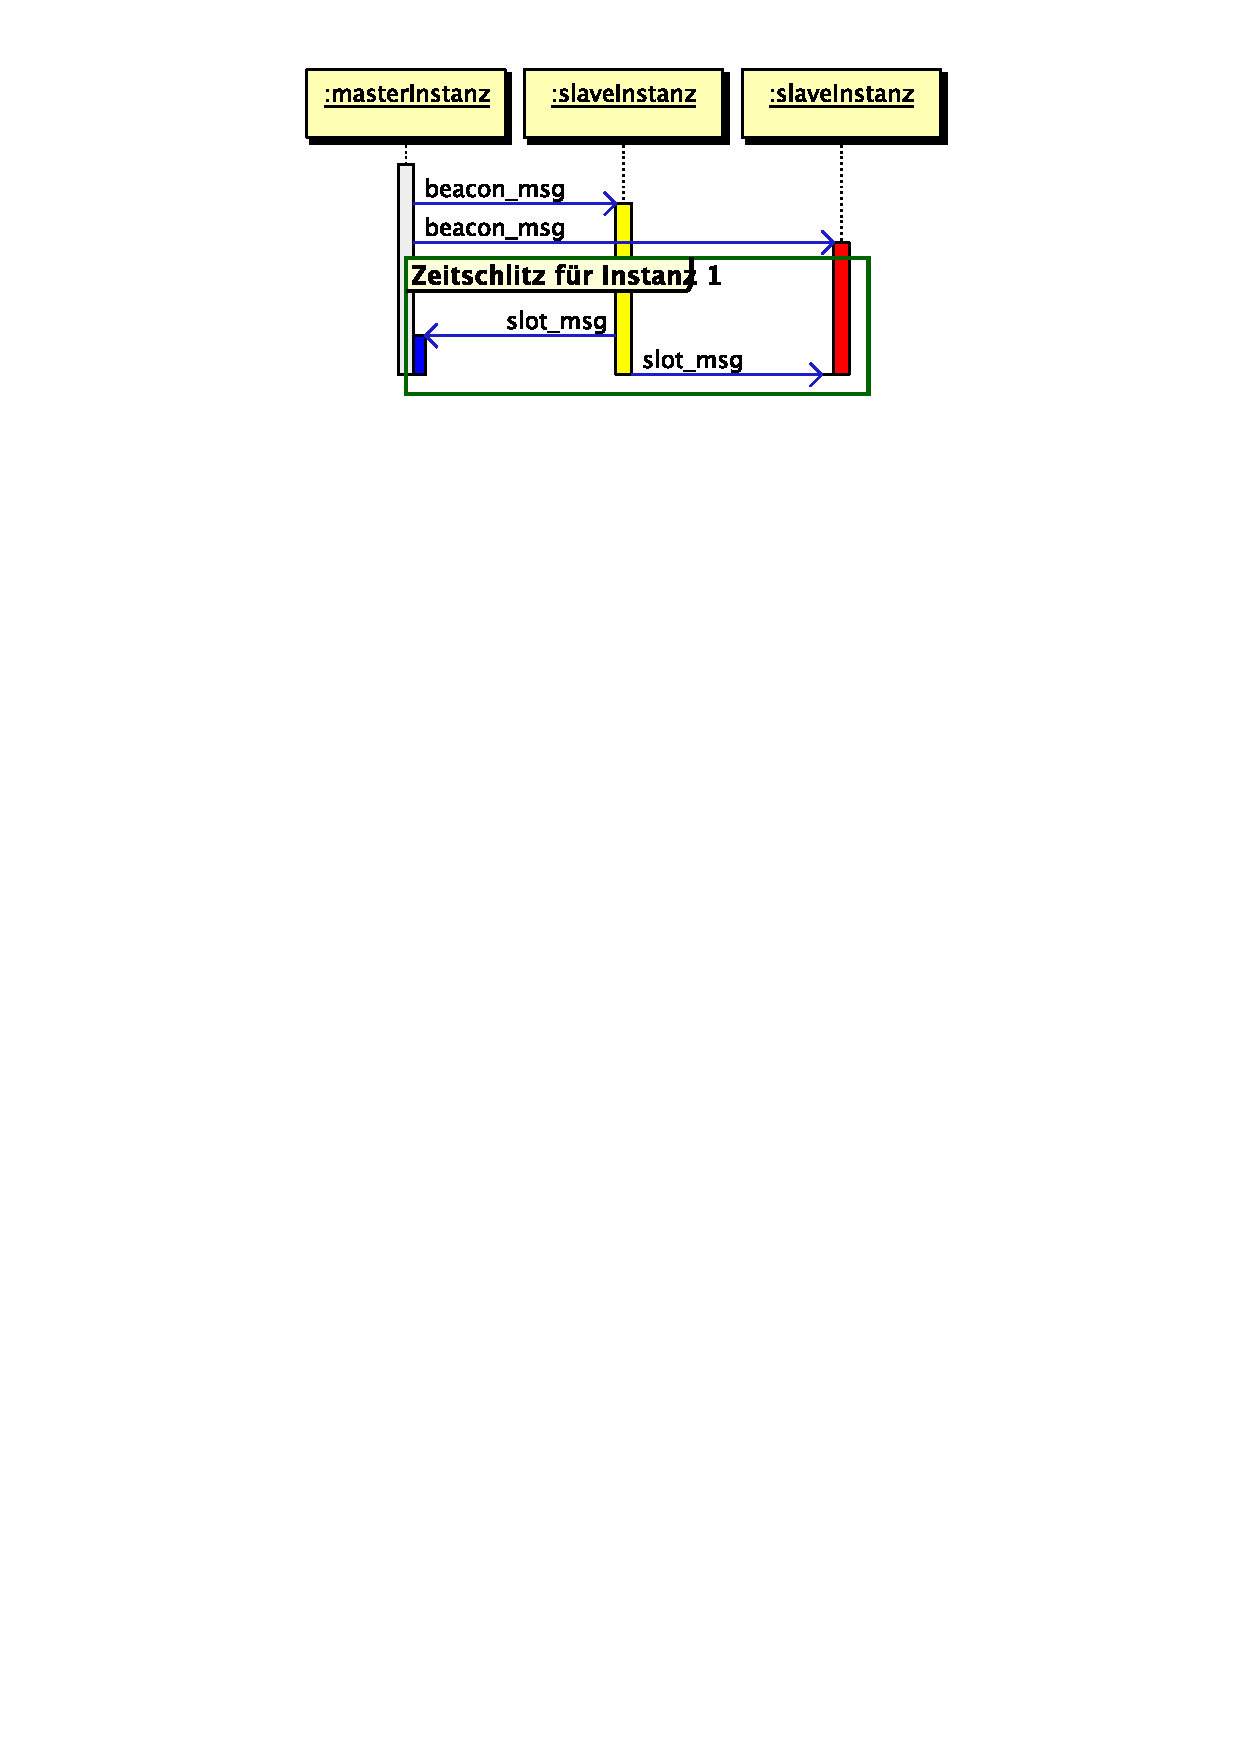
\includegraphics[scale=.75]{Documents/beacon_frame}
\end{center}

\end{document}
